\chapter{Laboratory measurement}
\subsection*{Stages in a measurement system}
\begin{figure}[H]
  \centering
  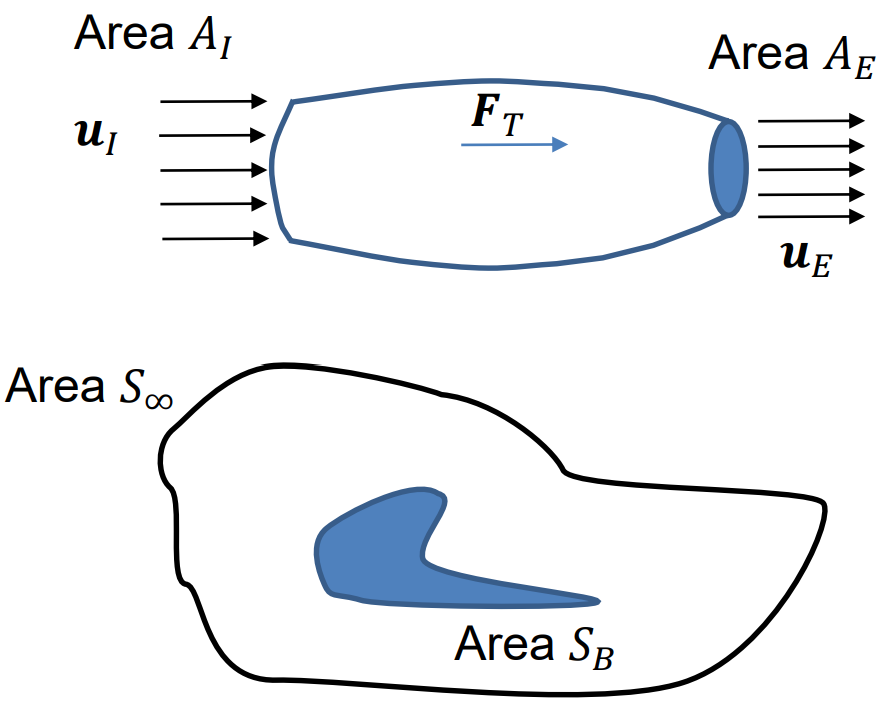
\includegraphics[width = 0.8 \textwidth]{./img/diagram38.png}
\end{figure}
\section{Amplifiers}
\begin{figure}[H]
  \centering
  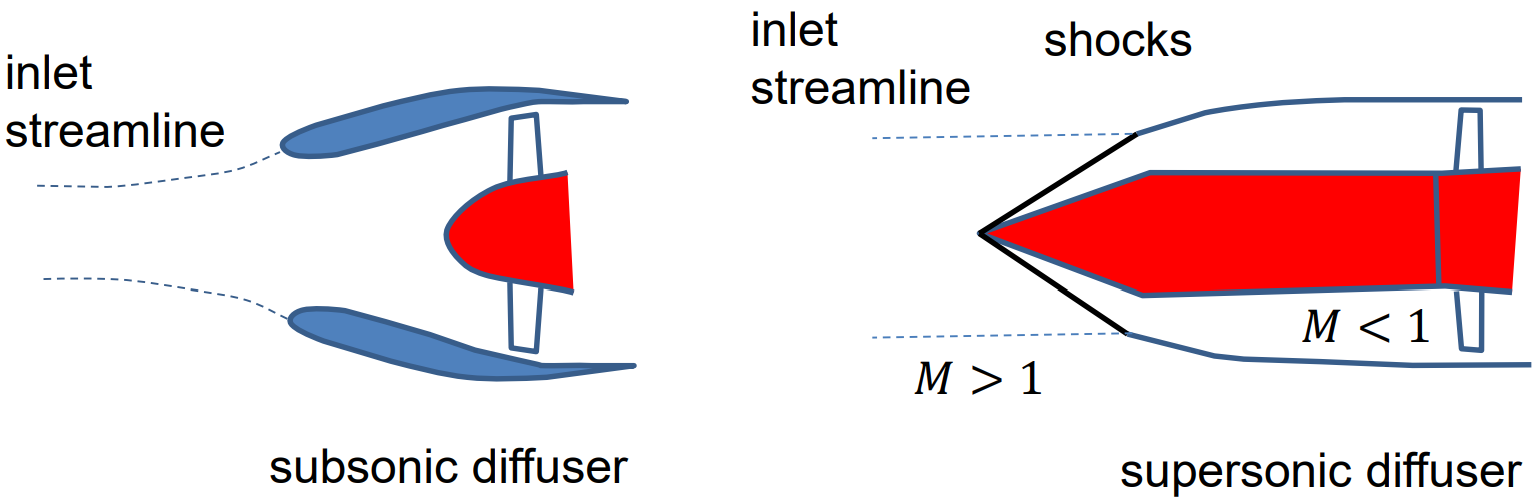
\includegraphics[width = 0.7\textwidth]{./img/diagram39.png}
\end{figure}
The voltage output from a transducer tends to be weak and this needs to be amplified. Operational amplifiers are normally around 1\si{\centi\meter} in size.
\begin{figure}[H]
  \centering
  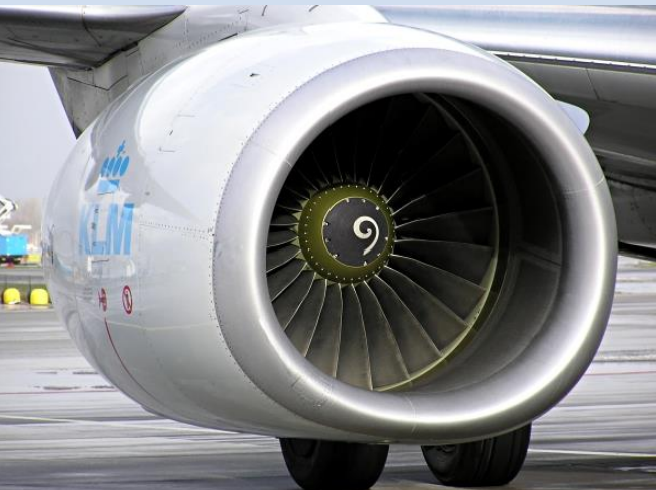
\includegraphics[width = 0.7\textwidth]{./img/diagram40.png}
\end{figure}
\begin{equation}
  V_0 = A_v (V_p - V_n) = A_v (V_2 - V_1)
\end{equation}
Where $A_v$ is the gain and $(V_p - V_n)$ can be from a Wheatstone bridge. Operational amplifiers are quite an old technology (since WW2) and are still used because they are cheap and convenient.
\begin{figure}[H]
  \centering
  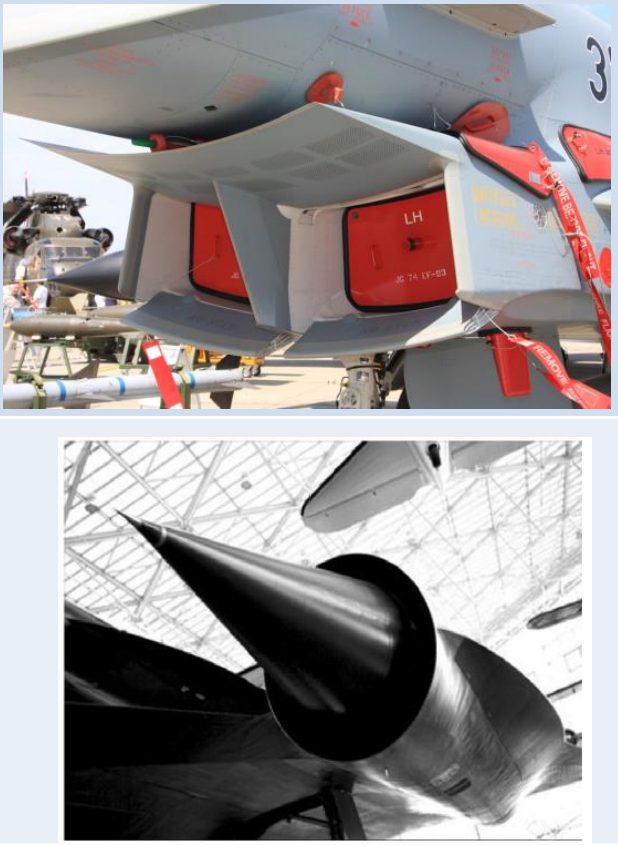
\includegraphics[width = 0.5\textwidth]{./img/diagram41.png}
\end{figure}
\begin{figure}[H]
  \centering
  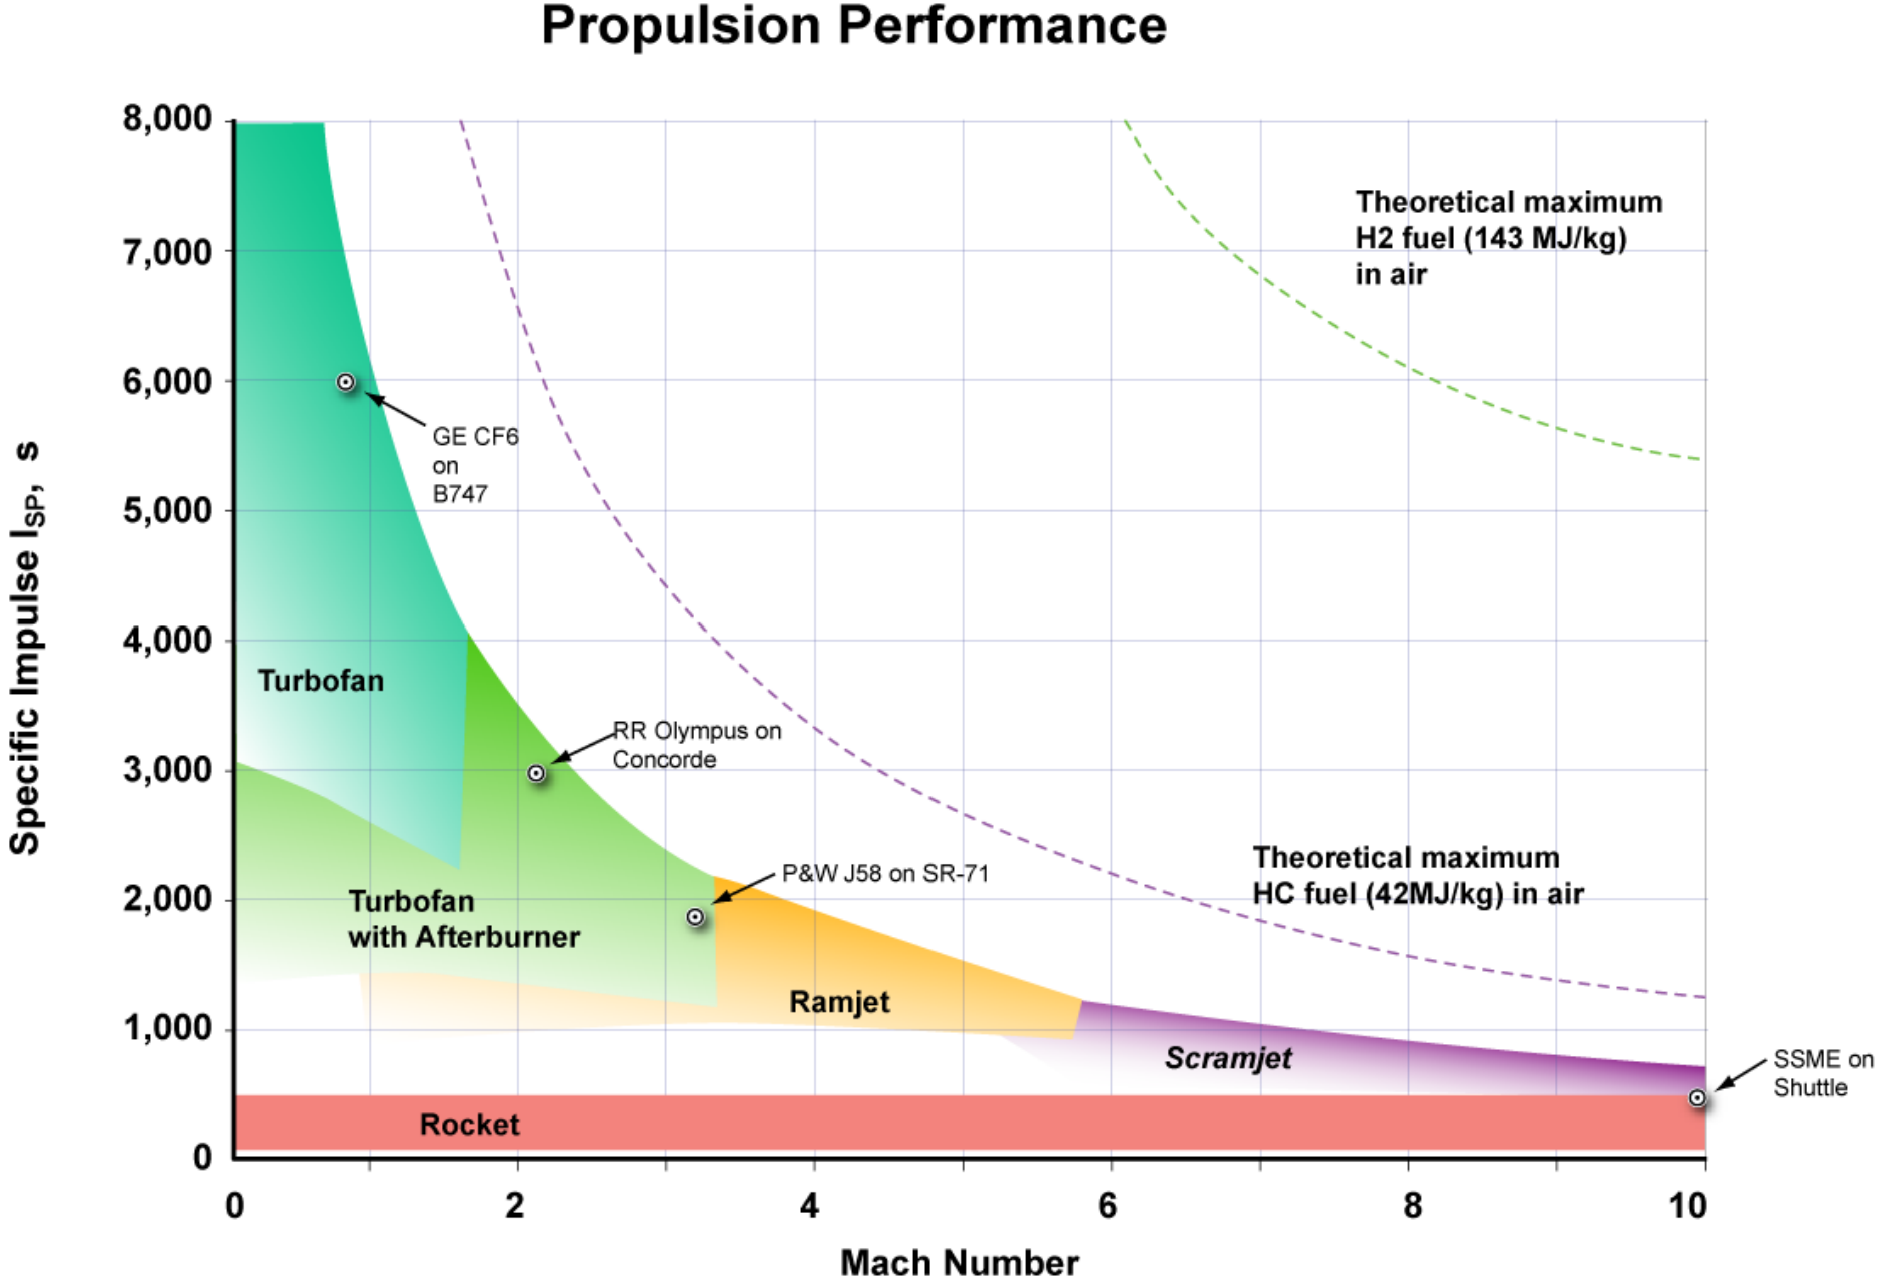
\includegraphics[width = 0.7\textwidth]{./img/diagram42.png}
\end{figure}
\subsection{Equivalent op-amp circuit and conditions of an ideal op-amp}
\begin{figure}[H]
  \centering
  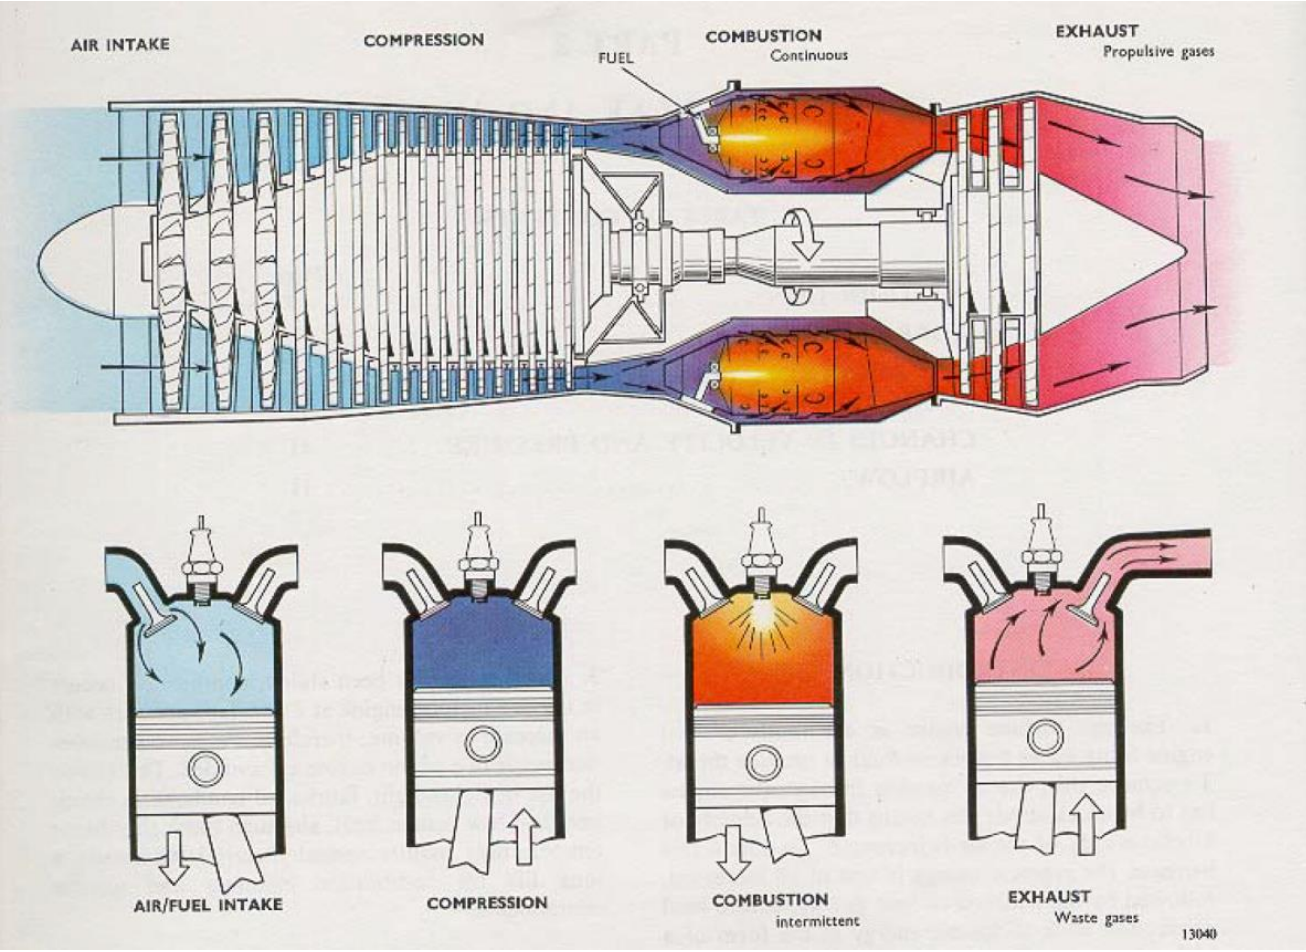
\includegraphics[width = 0.7\textwidth]{./img/diagram43.png}
\end{figure}
Terminology:
\begin{itemize}
  \item Differential input voltage: $V_i = V_p - V_n$
  \item Input resistance: $r_{in}$
  \item Output resistance: $r_{out}$
  \item Open-circuit output voltage: $V_{out}$
  \item Differential voltage gain: $A_v$
\end{itemize}
\begin{center}
  \begin{tabular}{ |c|c| }
    \hline
    \textbf{Conditions of an ideal op-amp}                             & \textbf{In reality}            \\
    \hline
    \hline
    No current into input terminals: $I_p = I_n = 0$                   &                                \\
    \hline
    Infinite input resistance: $r_{in} \rightarrow \infty$             & $r_{in} > 200 \si{\kilo \ohm}$ \\
    \hline
    Zero Output resistance $r_{out} = 0$                               & $r_{out} < 1 \si{\kilo\ohm}$   \\
    \hline
    Infinite differential (or open-loop) gain $A_v \rightarrow \infty$ & $A_v > 100000$                 \\
    \hline
    Zero common-mode voltage gain $A_{cm} = 0$                         & $A_v$ also frequency dependant \\
    \hline
  \end{tabular}
\end{center}
\subsection{Non-zero voltage with zero current?}
\begin{figure}[H]
  \centering
  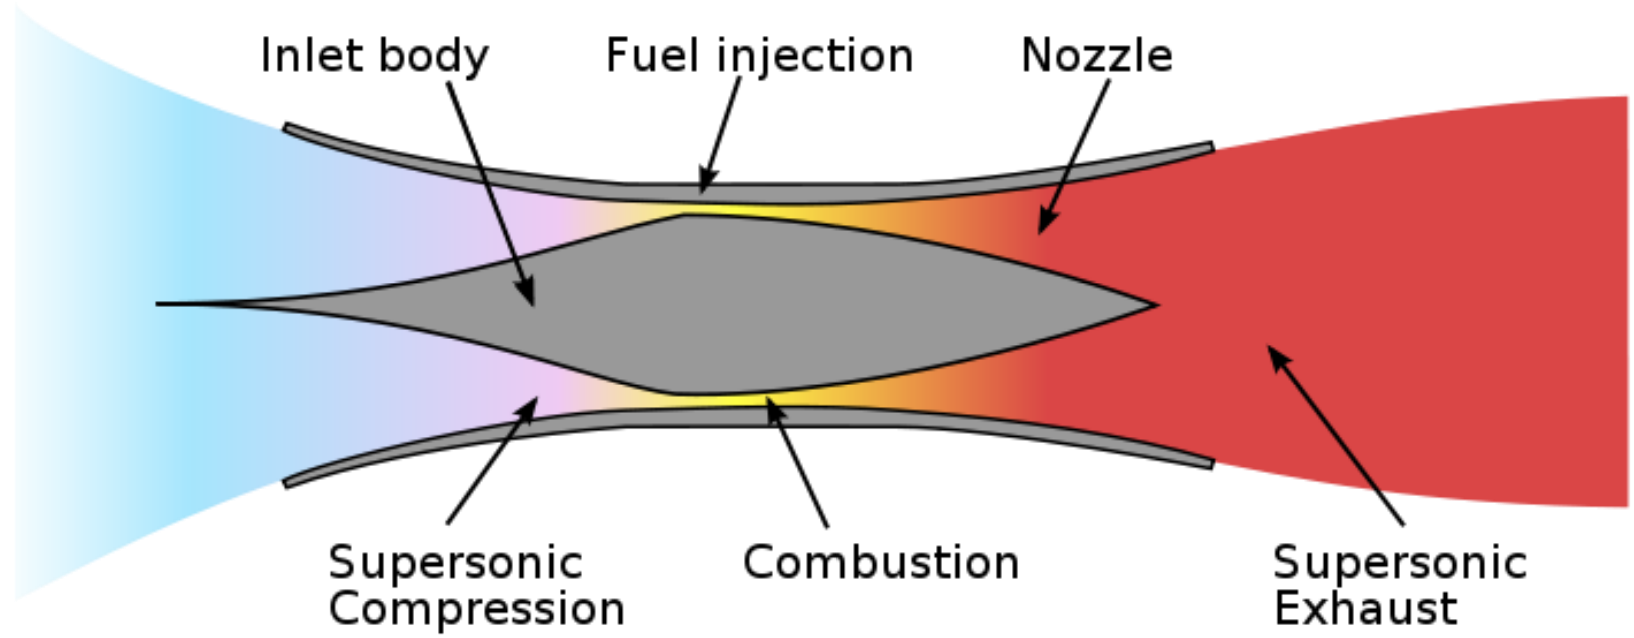
\includegraphics[width = 0.7\textwidth]{./img/diagram44.png}
\end{figure}
A question that is often asked is if the current is zero, how can we still have a voltage? When you connect a battery to a meter, where the meter resistance is normally huge. We can still measure the voltage. This is due to Ohm's law $I = \frac{V}{R_m}$. A good analogy to make is a plunger system, where the other end is covered. When you push down, increasing the pressure, this can still be felt on the tip of the thumb, despite there being no flow. In the same way, we can still 'feel' the voltage with 'no' current flow.
\subsection{Saturation}
In a practical scenario, we want to strengthen the weak signal from the sensor. Let us connect an input to the non-inverting terminal and the inverting input to the ground.
\begin{figure}[H]
  \centering
  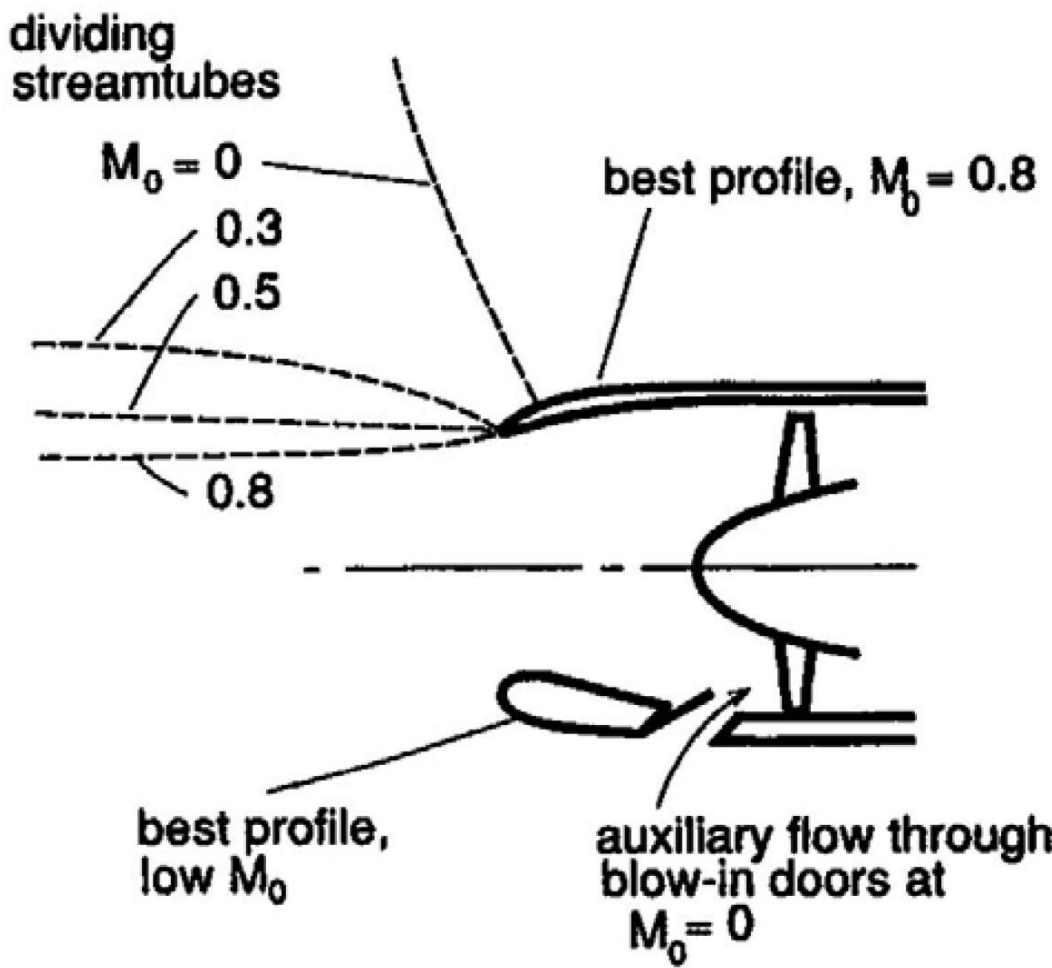
\includegraphics[width = 0.7\textwidth]{./img/diagram45.png}
\end{figure}
We can see that the signal is not infinitely amplified, as we are limited by the energy provided by our supply voltage. This is reflected in the graph above as the straight portion of the amplified line. This is called saturation. Due to $A_v$ being quite large, our linear region is normally tiny. This may be a problem if we want to measure the linear region.
\subsection{Negative feedback}
So op-amps seem to be a useful device but also seem to be a bit tricky. They are much more useful when used as part of a larger circuit. Negative feedback is achieved by feeding a fraction of the output signal back to the \textbf{inverting} terminal as shown. By definition, the closed-loop gain of such a device is:
\begin{equation}
  G = \frac{V_0}{V_i}
\end{equation}
\begin{figure}[H]
  \centering
  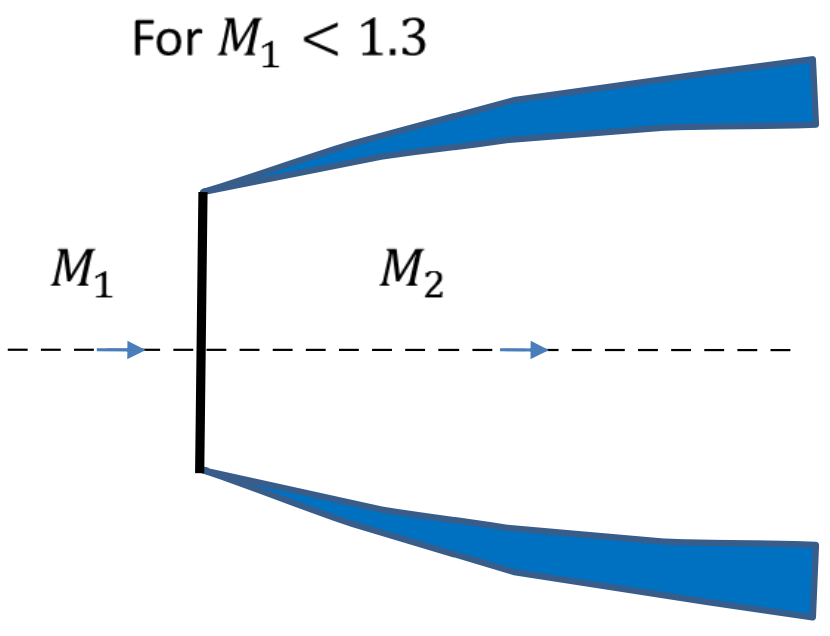
\includegraphics[width = 0.5\textwidth]{./img/diagram46.png}
\end{figure}
Negative feedback trades a reduction in gain with one that is smaller, stable and predictable, whilst giving the designer control over operational characteristics.
\subsection{Basic feedback amplifier configurations}
Only 2 resistors are required to construct a negative feedback amplifier. Note that output signal is always fed-back to the inverting input terminal.
\begin{figure}[H]
  \centering
  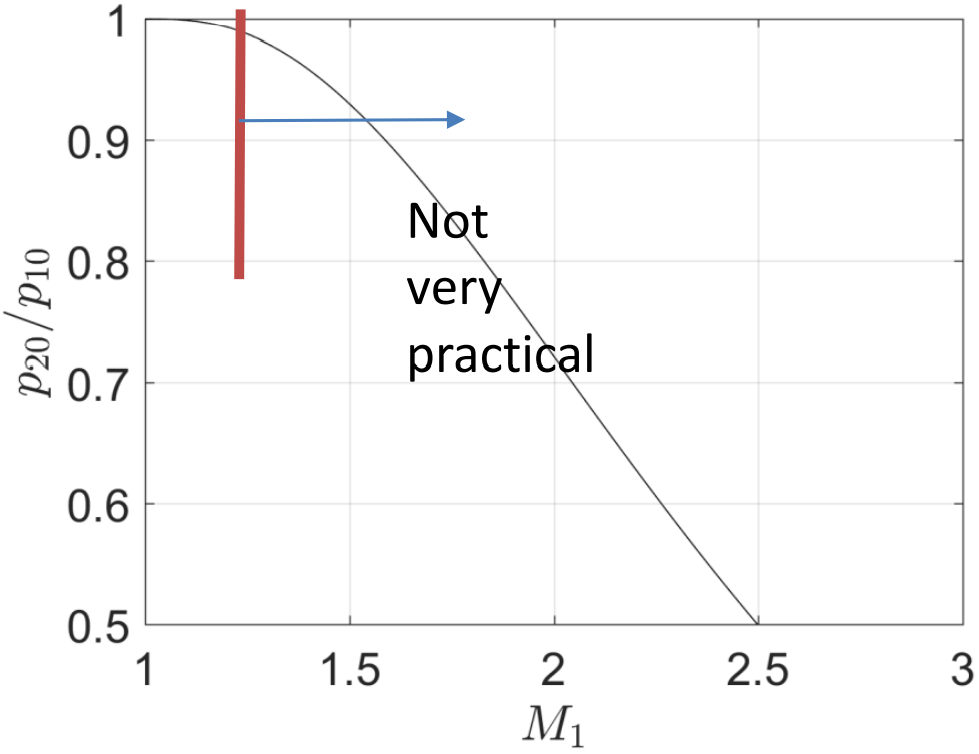
\includegraphics[width = 0.5\textwidth]{./img/diagram47.png}
  \caption{Inverting feedback amplifier arrangement.}
\end{figure}
\begin{figure}[H]
  \centering
  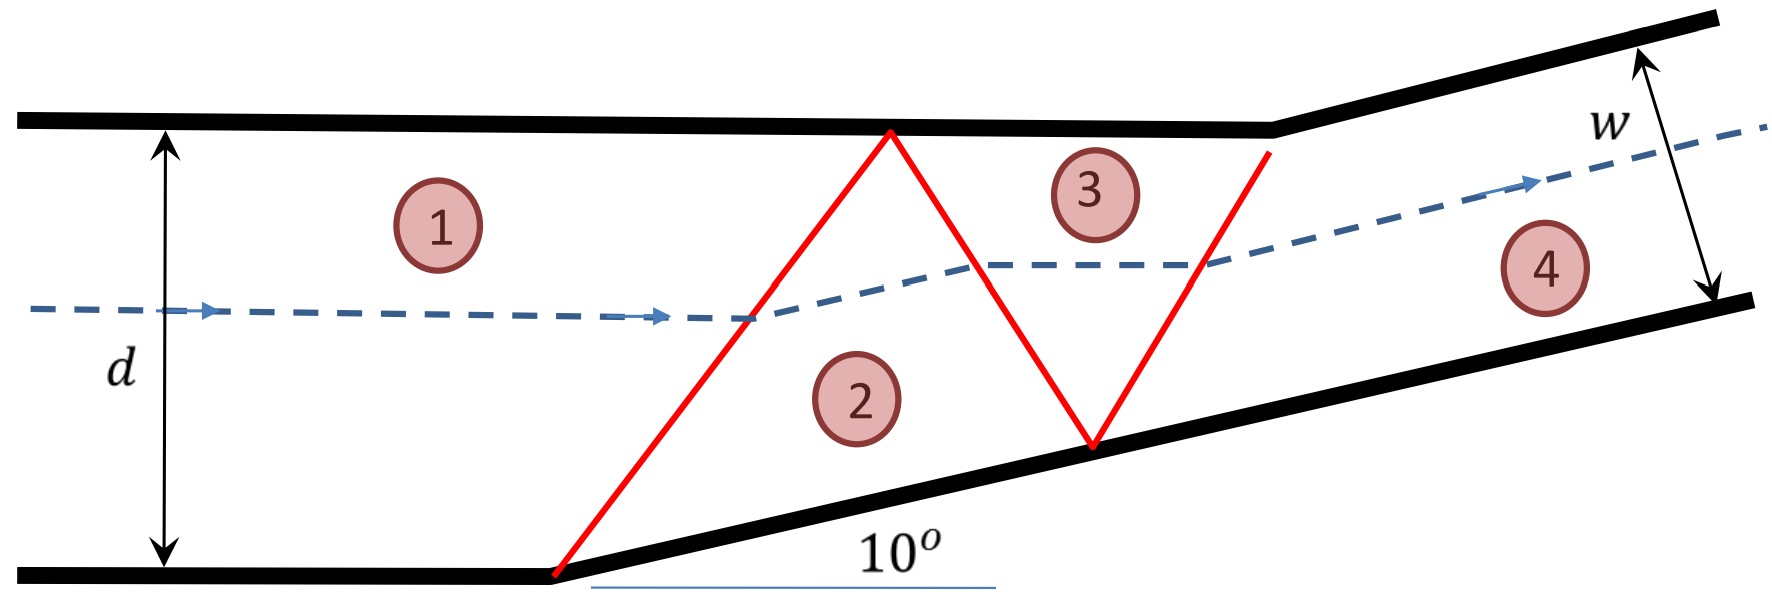
\includegraphics[width = 0.5\textwidth]{./img/diagram48.png}
  \caption{Non-inverting feedback amplifier arrangement.}
\end{figure}
We can see the difference between an inverting and non-inverting feedback amplifier is which input the source signal is connected to.
\subsection{Basic inverting feedback amplifier}
\begin{figure}[H]
  \centering
  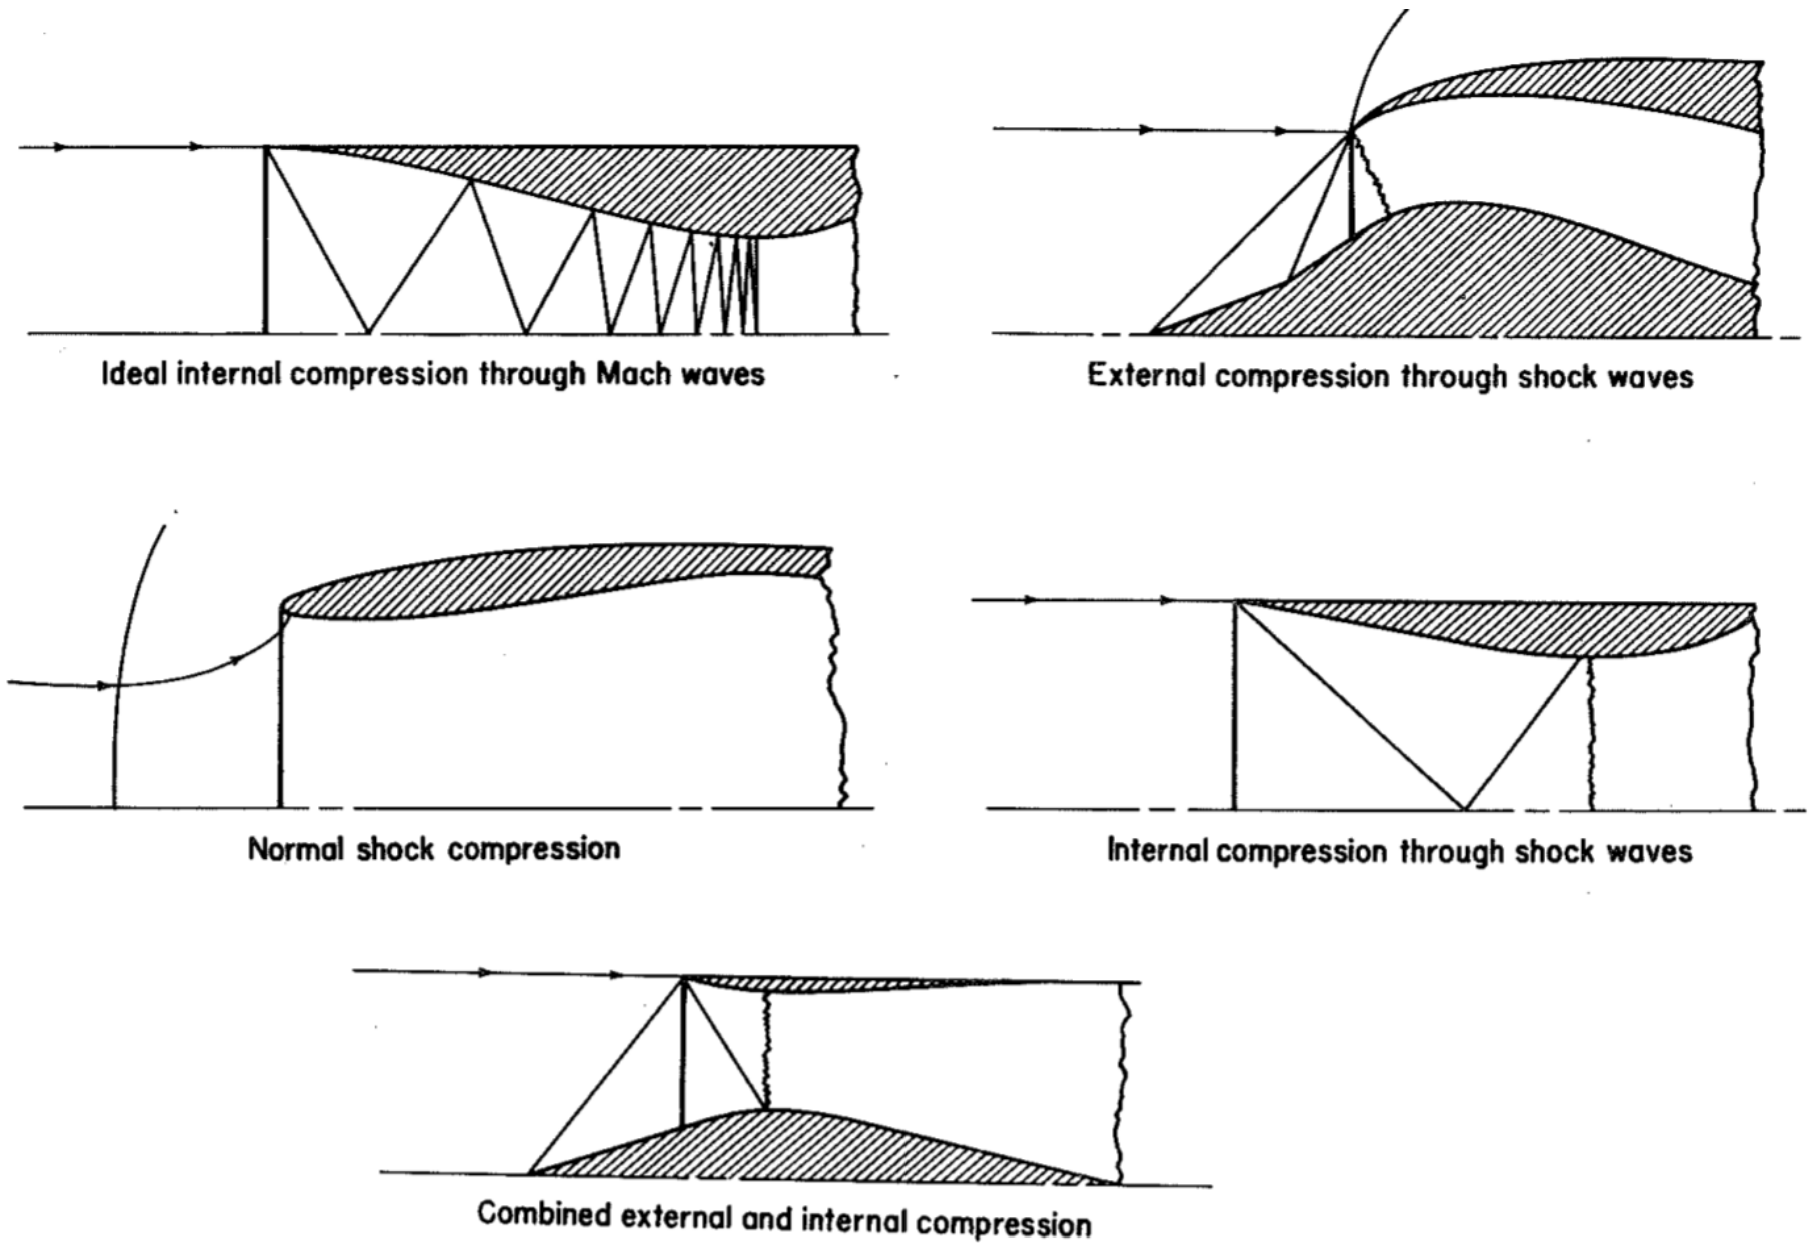
\includegraphics[width = 0.5\textwidth]{./img/diagram49.png}
\end{figure}
Let us derive its closed loop gain $G$. By definition:
\begin{gather}
  V_0 = A_v(V_p - V_n)\\
  V_p \rightarrow 0 \Longrightarrow V_n = - \frac{V_0}{A_v} \label{invertingfb1}
\end{gather}
Apply KCL to Node 1:
\begin{gather}
  \frac{V_{in}-V_n}{R_1} - I_n - \frac{V_n - V_0}{R_2} = 0 \Longrightarrow \frac{R_2}{R_1}V_{in} + v_n \left( 1 + \frac{R_2}{R_1} \right) = V_0 \label{invertingfb2}
\end{gather}
$I_n$ is 0 from our model assumptions.
Combining equations (\ref{invertingfb1}) and (\ref{invertingfb2}), we arrive at:
\begin{gather}
  G \equiv \frac{V_0}{V_{in}} = -\frac{R_2}{R_1} \frac{1}{1 + \frac{1}{A_v}\left( 1 + \frac{R_2}{R_1}\right)}
\end{gather}
For an ideal op-amp, $A_v \rightarrow \infty$:
\begin{equation}
  G = \frac{V_0}{V_{in}} = - \frac{R_2}{R_1}
\end{equation}
\subsection{Basic non-inverting feedback amplifier}
\begin{figure}[H]
  \centering
  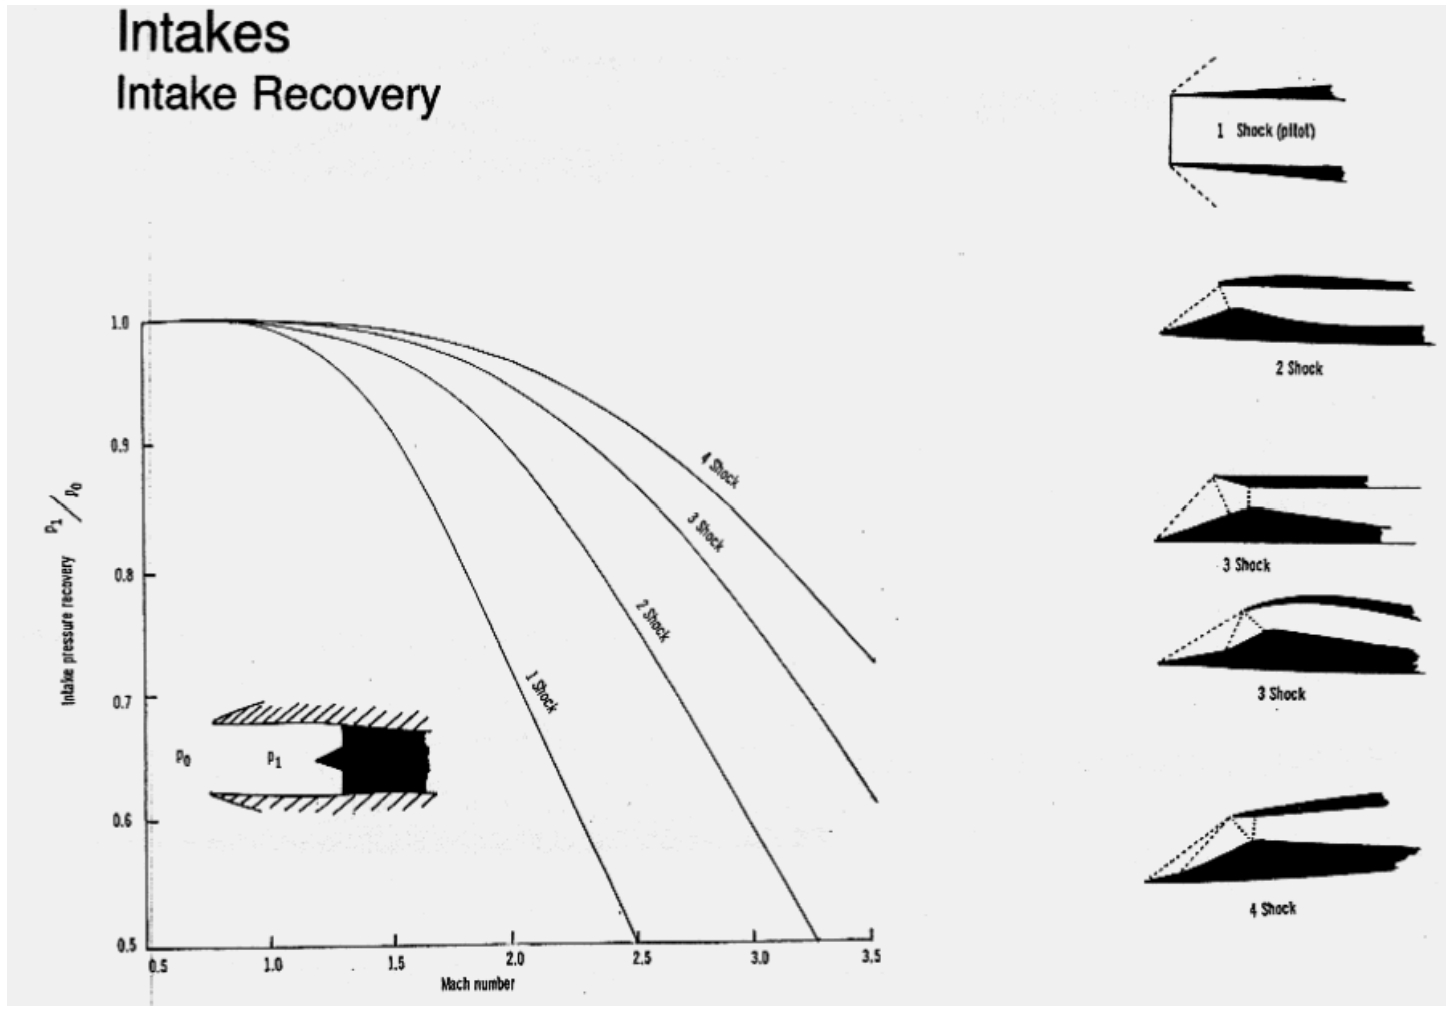
\includegraphics[width = 0.5\textwidth]{./img/diagram50.png}
\end{figure}
Derive its closed-loop gain $G$. By definition:
\begin{equation}
  V_0 = A_v (V_p - V_n) \label{noninvertingfb1}
\end{equation}
Apply KCL to node 1
\begin{gather}
  \frac{0 - V_n}{R_1} = \frac{V_n - V_0}{R_2} \rightarrow \frac{V_0}{R_2} = V_n \left(\frac{1}{R_1} + \frac{1}{R_2}\right) \label{noninvertingfb2}
\end{gather}
Combining equation (\ref{noninvertingfb1}) and (\ref{noninvertingfb2}), we arrive at:
\begin{equation}
  G \equiv \frac{V_0}{V_{in}} = \frac{1 + \frac{R_2}{R_1}}{1 + \frac{1}{A_v}\left(1 + \frac{R_2}{R_1}\right)}
\end{equation}
For an ideal amplifier, $A_v \rightarrow \infty$:
\begin{equation}
  G = 1 + \frac{R_2}{R_1}
\end{equation}
This is positive and always greater than 1.
\subsection{Summary}
\subsubsection*{Ideal feedback amplifier characteristics}
\begin{center}
  \begin{tabularx}{0.8\textwidth} {
      | >{\centering\arraybackslash}X
      | >{\centering\arraybackslash}X
      | >{\centering\arraybackslash}X |}
    \hline
                             & \textbf{Inverting amplifier} & \textbf{Non-inverting amplifier} \\
    \hline
    \hline
    $G = \frac{V_0}{V_{in}}$ & $-\frac{R_2}{R_1}$           & $1 + \frac{R_2}{R_1}$            \\
    \hline
    $R_{in}$                 & $R_1$                        & $\infty$                         \\
    \hline
    $R_{out}$                & 0                            & 0                                \\
    \hline
  \end{tabularx}
\end{center}
\subsection{Voltage amplification summary}
Operational amplifier:
\begin{itemize}
  \item The gain usually is too large (typically $>$ 100,000) and not well defined. ($V_0$ cannot be larger than supply voltage)
  \item The gains for two op-amps of the same type can differ by a factor of two or more.
  \item The gain is not stable, can change with temperature, can change with changes of supply voltage.
\end{itemize}
To reduce these effects, we use negative feedback.
\begin{figure}[H]
  \centering
  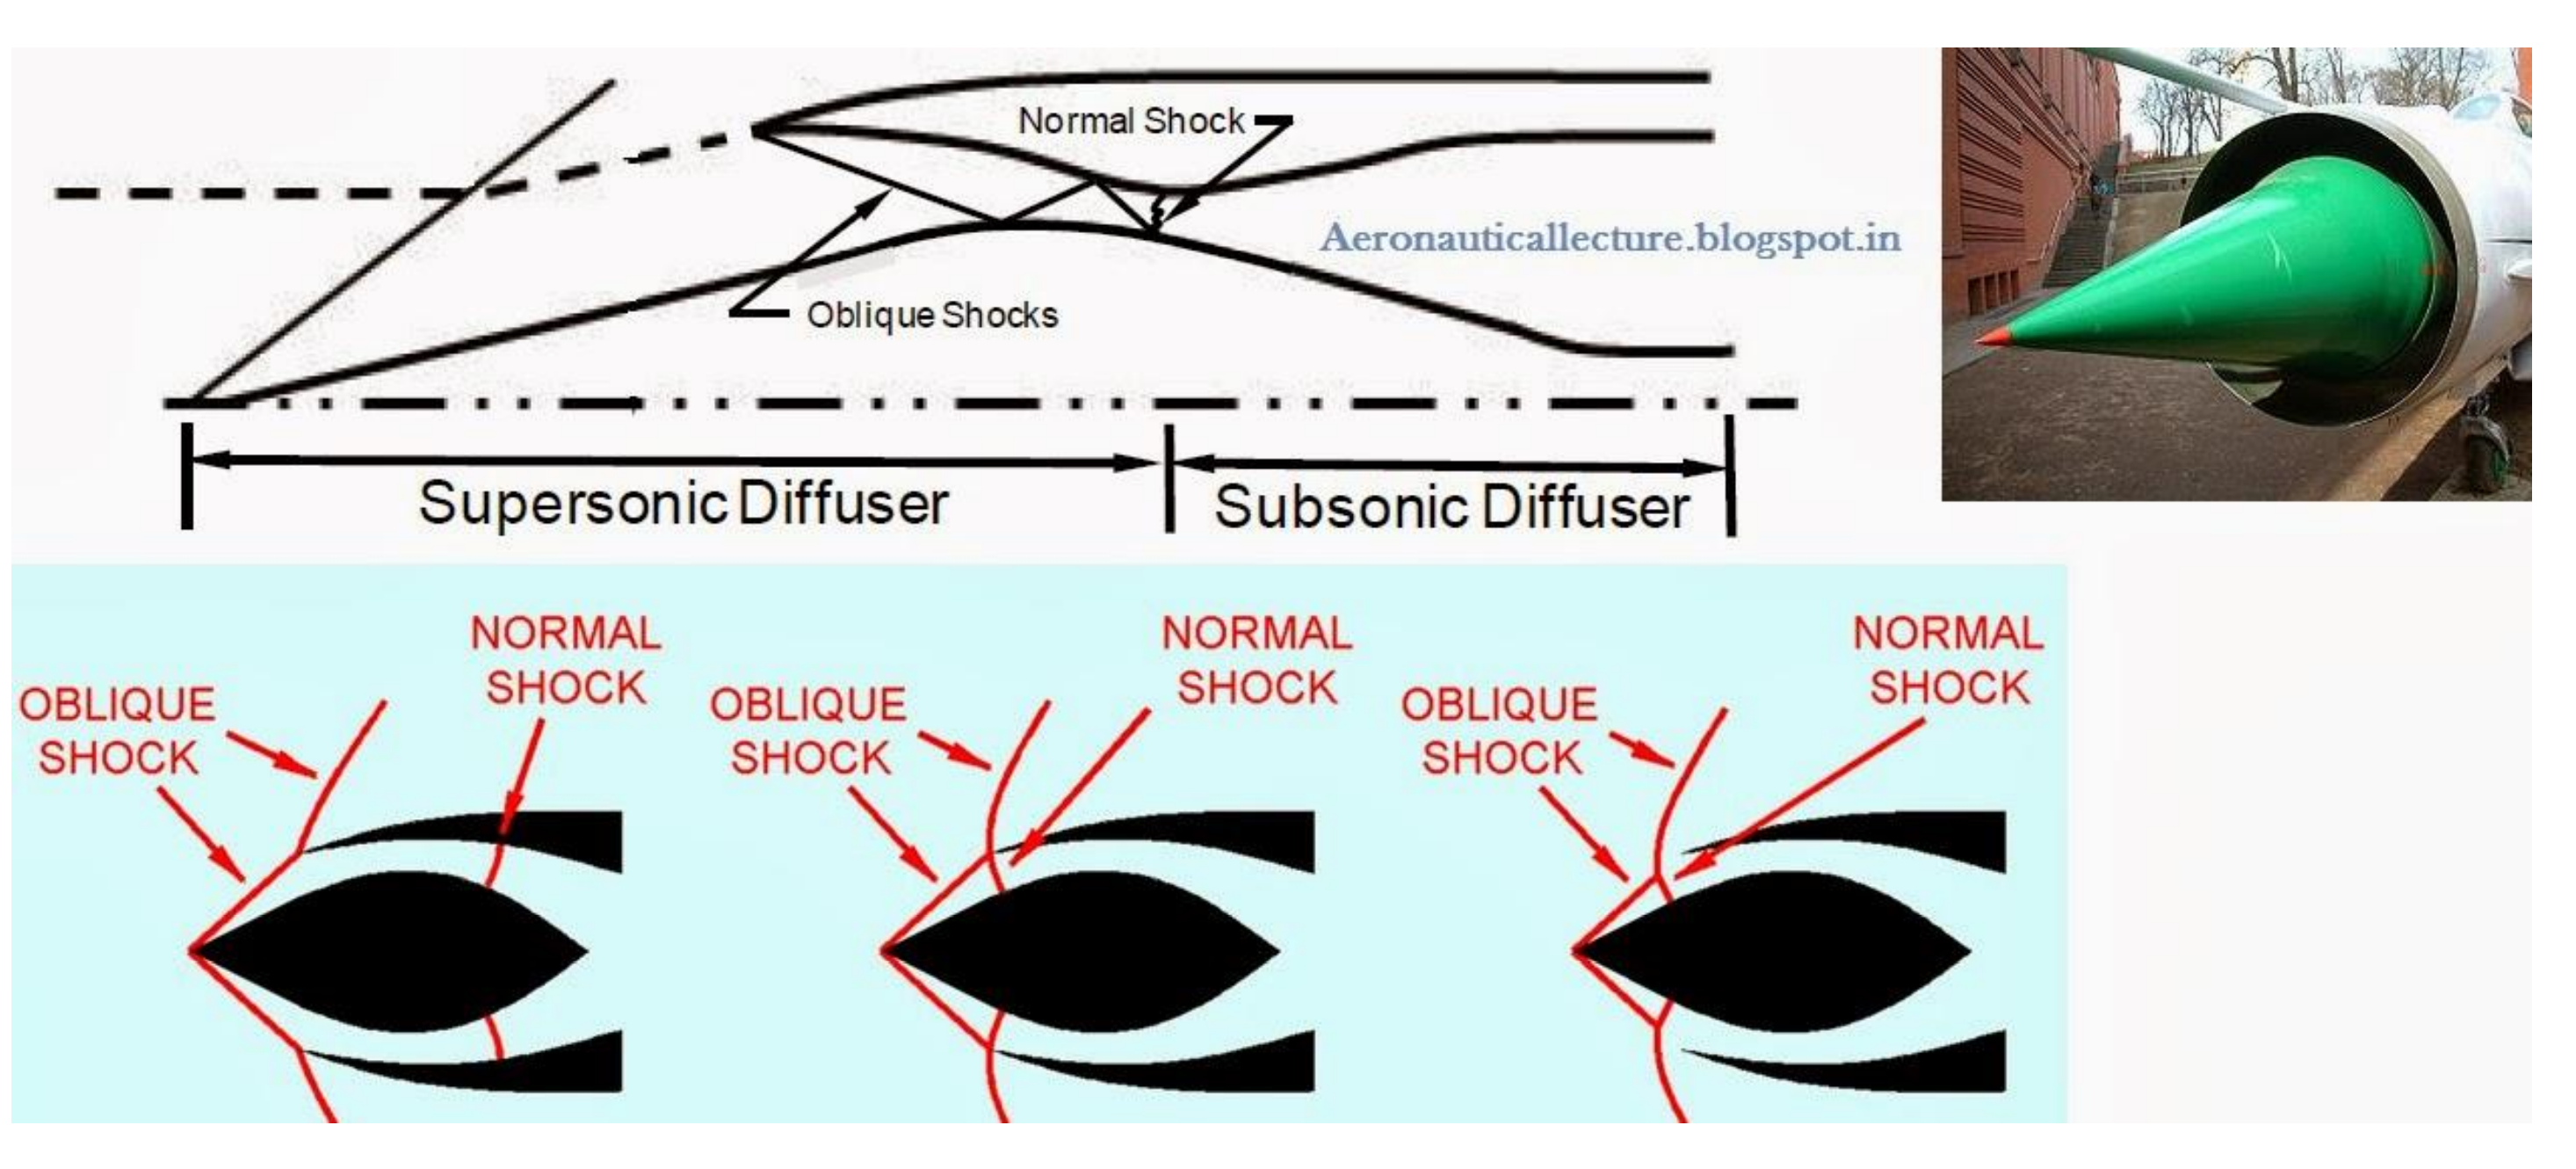
\includegraphics[width = 0.5\textwidth]{./img/diagram51.png}
  \caption{$V_1$ and $V_2$ could come from a Wheatstone bridge.}
\end{figure}
The output voltage $V_0$ is given as:
\begin{gather}
  V_0 = \frac{R_F}{R_1}(V_2 - V_1)
\end{gather}
Only when $\frac{R_3}{R_2} = \frac{R_F}{F_1}$. This is independent of $A_v$ and the gain of this circuit, $G = \frac{R_F}{R_1}$ is well controllable.
\subsection{Difference amplifier}
Combining a non-inverting and inverting op-amp to take the difference between two inputs:
\begin{figure}[H]
  \centering
  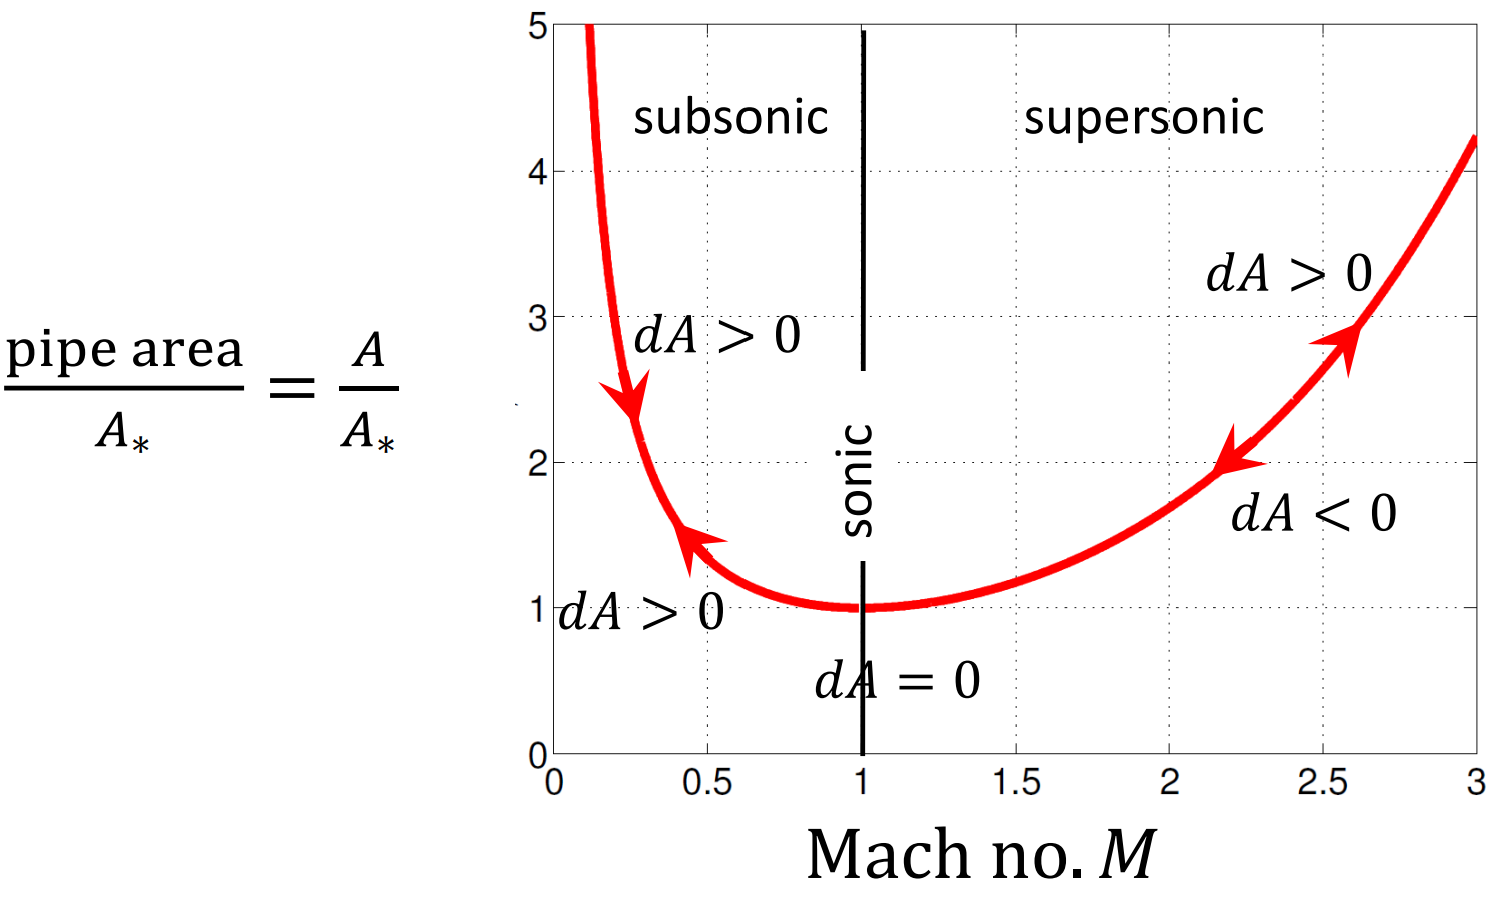
\includegraphics[width = 0.5\textwidth]{./img/diagram52.png}
\end{figure}
\begin{gather}
  \frac{V_0}{A_v} = V_+ - V_- \rightarrow 0 \textrm{ as } A_v \rightarrow \infty\\
  V_+ = \frac{R_3}{R_2 + R_3} \leftarrow \textrm{ voltage divider} \label{difamp1}
\end{gather}
KCL at node N1
\begin{gather}
  \frac{V_0 - V_-}{R_f} = \frac{V_- V_1}{R_1} \rightarrow \frac{V_0}{R_f} + \frac{V_1}{R_1} = \left(\frac{1}{R_f} + \frac{1}{R_1}\right)V_-\\
  \frac{V_0}{R_f} + \frac{V_1}{R_1} = \left(\frac{R_f + R_1}{R_f R_1}\right)\left(\frac{R_3}{R_2 + R_3}\right)V_2 \label{difamp2}
\end{gather}
Combining equation (\ref{difamp1}) and (\ref{difamp2}), we arrive at:
\begin{gather}
  V_0 = R_f \left(\frac{R_f + R_1}{R_f R_1}\right)\left(\frac{R_3}{R_2 + R_3}\right)V_2 - \frac{R_f}{R_1} V_1\\
  V_0 = \frac{1 + \frac{R_f}{R_1}}{1 + \frac{R_2}{R_3}}V_2 - \frac{R_f}{R_1}V_1
\end{gather}
If we can make sure that $\frac{R_f}{R_1} = \frac{R_3}{R_2}$ is satisfied, we can further reduce our equation to:
\begin{gather}
  V_0 = \frac{R_f}{R_i}(V_2 - V_1)
\end{gather}
\subsection{On a bread board}
\begin{figure}[H]
  \centering
  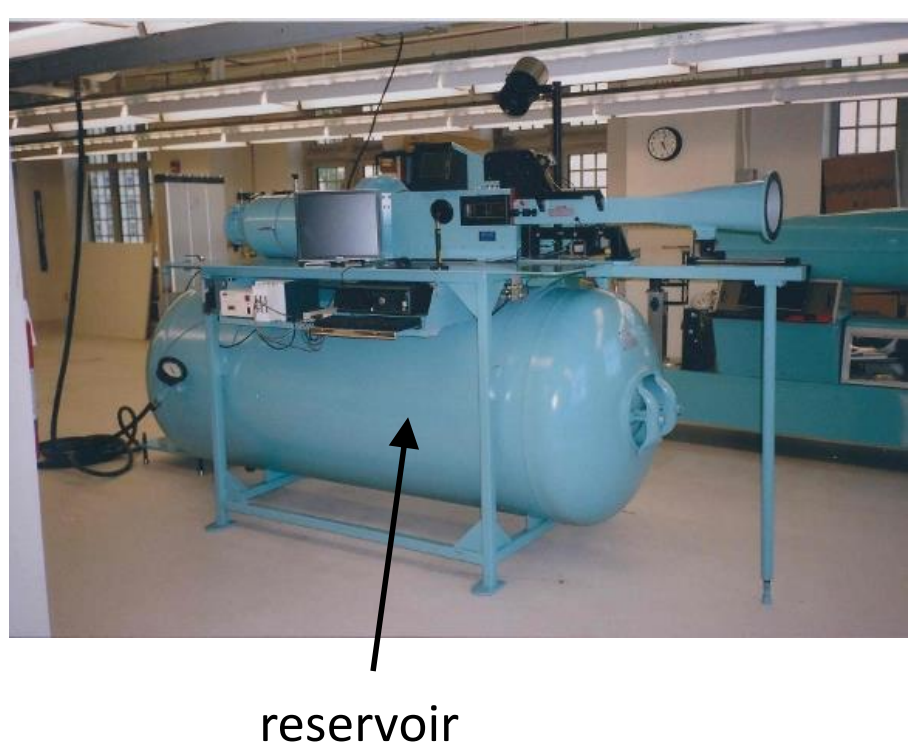
\includegraphics[width = 0.8\textwidth]{./img/diagram53.png}
\end{figure}
\begin{equation}
  V_0 = \frac{R_f}{R_i}(R_2 - R_1)
\end{equation}
if $\frac{R_f}{R_1} = \frac{R_3}{R_2}$ can be satisfied.
\section{Analogue-Digital (AD) conversion}
\begin{figure}[H]
  \centering
  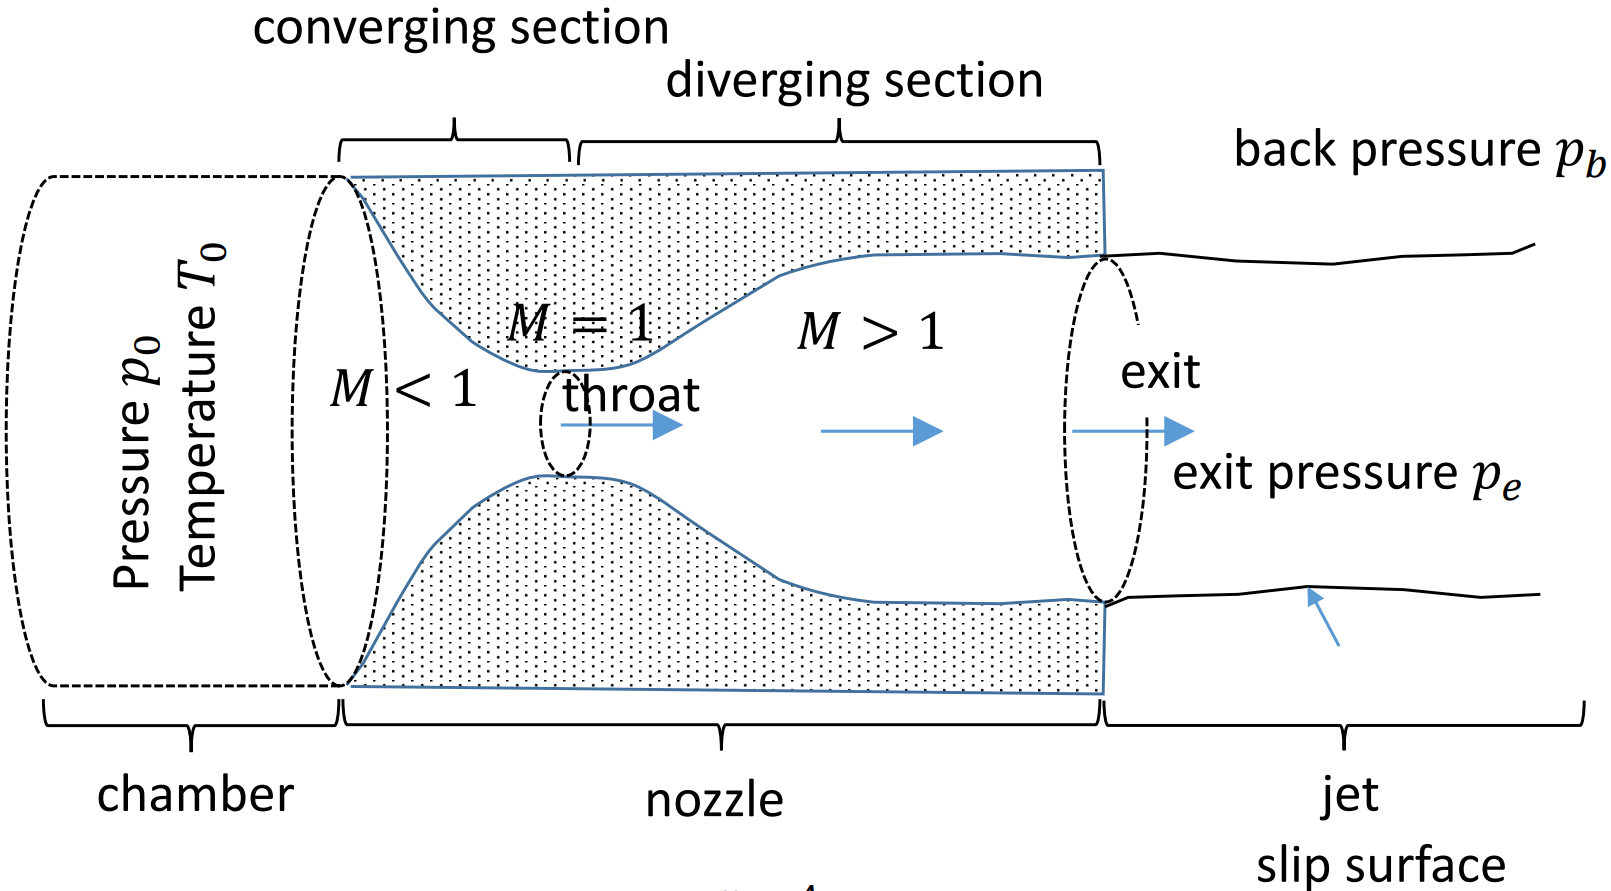
\includegraphics[width = 0.8\textwidth]{./img/diagram54.png}
\end{figure}
\subsection{Comparator}
We are using an op-amp here, because when we have a high $A_v$, we have a very small linear region. Hence, when we look at a signal graph, we can see this as a sort of switching device:
\begin{figure}[H]
  \centering
  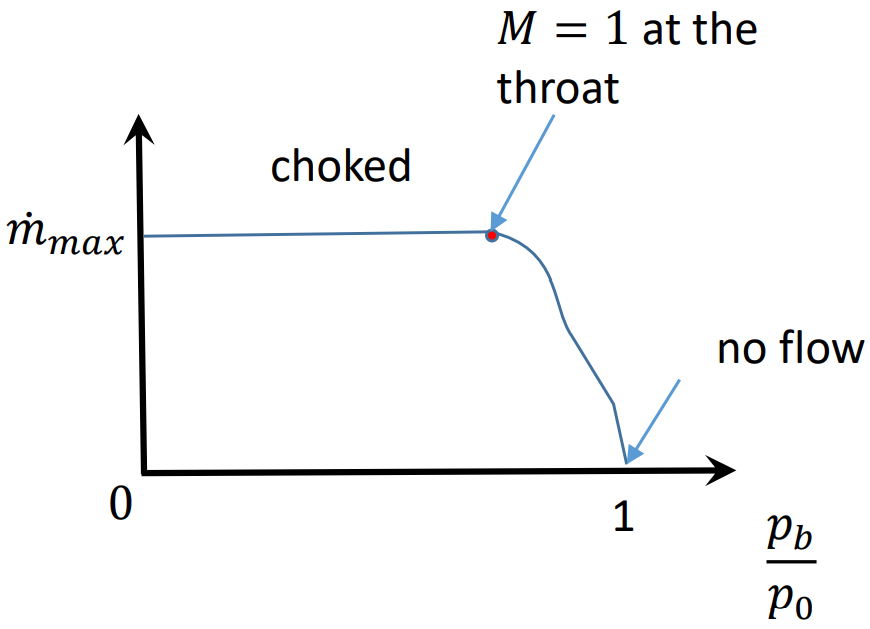
\includegraphics[width = 0.8\textwidth]{./img/diagram55.png}
\end{figure}
With very large $A_v$, output $V_0$ would be: $V_0 = A_v (V_p - V_n)$. Hence:
\begin{equation}
  V_0 \begin{cases}
    = VCC \textrm{ ... if } V_p > V_n \\
    = VEE \textrm{ ... if } V_p < V_n
  \end{cases}
\end{equation}
This essentially makes comparisons based on $V_p$ and $V_n$
\begin{equation}
  V_p > V_n \ ? \rightarrow \textrm{YES/NO}
\end{equation}
\subsection{Example ADC mechanism using comparators}
A circuit to compare voltages:
\begin{figure}[H]
  \centering
  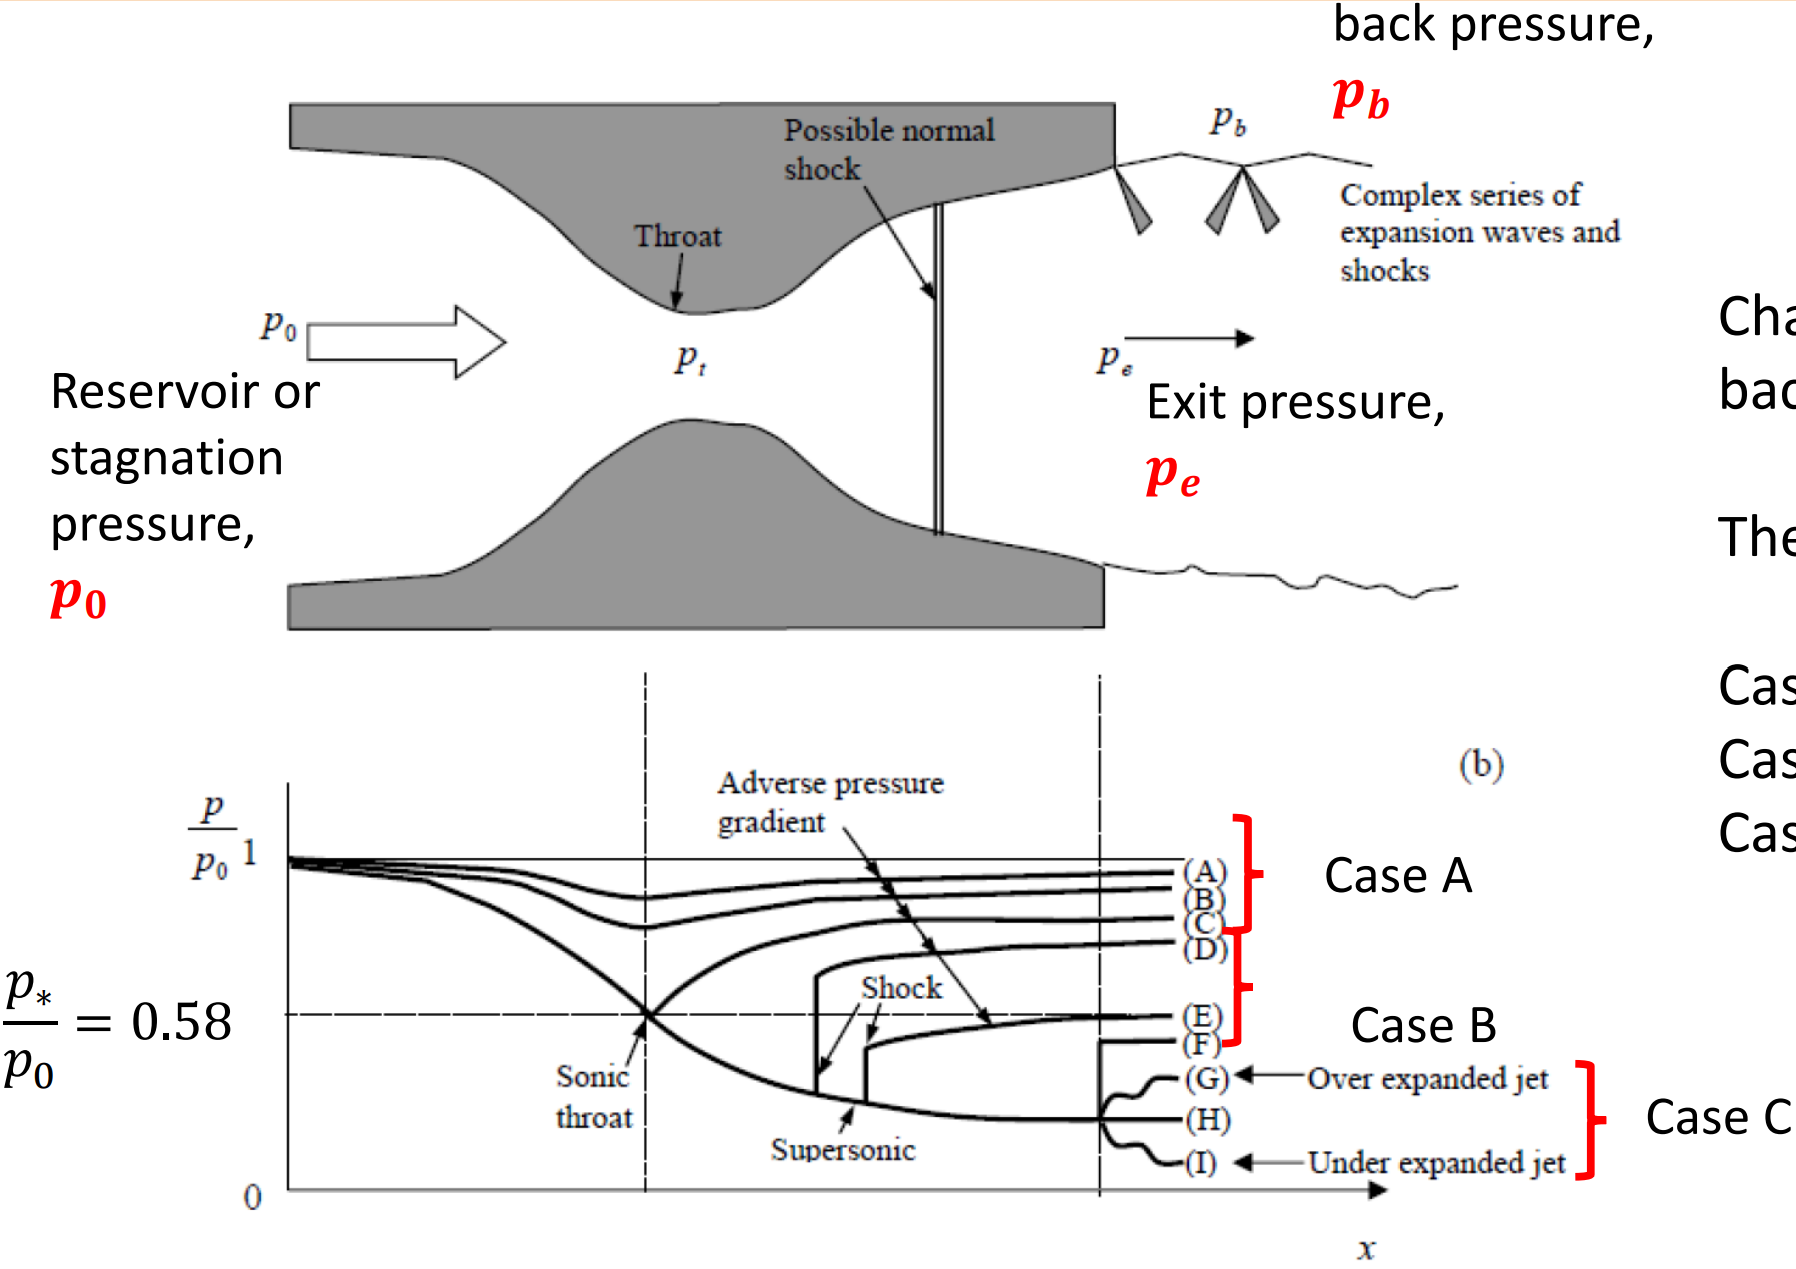
\includegraphics[width = 0.4\textwidth]{./img/diagram56.png}
  \caption{\textbf{Flash ADC:} number of comparisons done in parallel.}
\end{figure}
Setting up these comparators in parallel and setting a reference voltage for each, we can compare a single input and produce a digital binary signal, which tells us the range of voltages that $V_{in}$ may occupy. In this case we can see that:
\begin{equation}
  2.1 \si{\volt} < V_{in} < 2.2 \si{\volt}
\end{equation}
Hence, $V_{in}$ may be 2.1\si{\volt}, but other options are possible. When we store in a digital binary format this is called \textbf{quantisation}. When a voltage range 0-5\si{\volt} ($V_{REF} = 5\si{\volt}$) is quantised in 8-bit,
\begin{equation}
  V_{in} = 2.14\si{\volt} \rightarrow V_{\textrm{in, quantised}} = int \left(\frac{V_{in}}{5[\si{\volt}]/2^8}\right) = 110
\end{equation}
\begin{figure}[H]
  \centering
  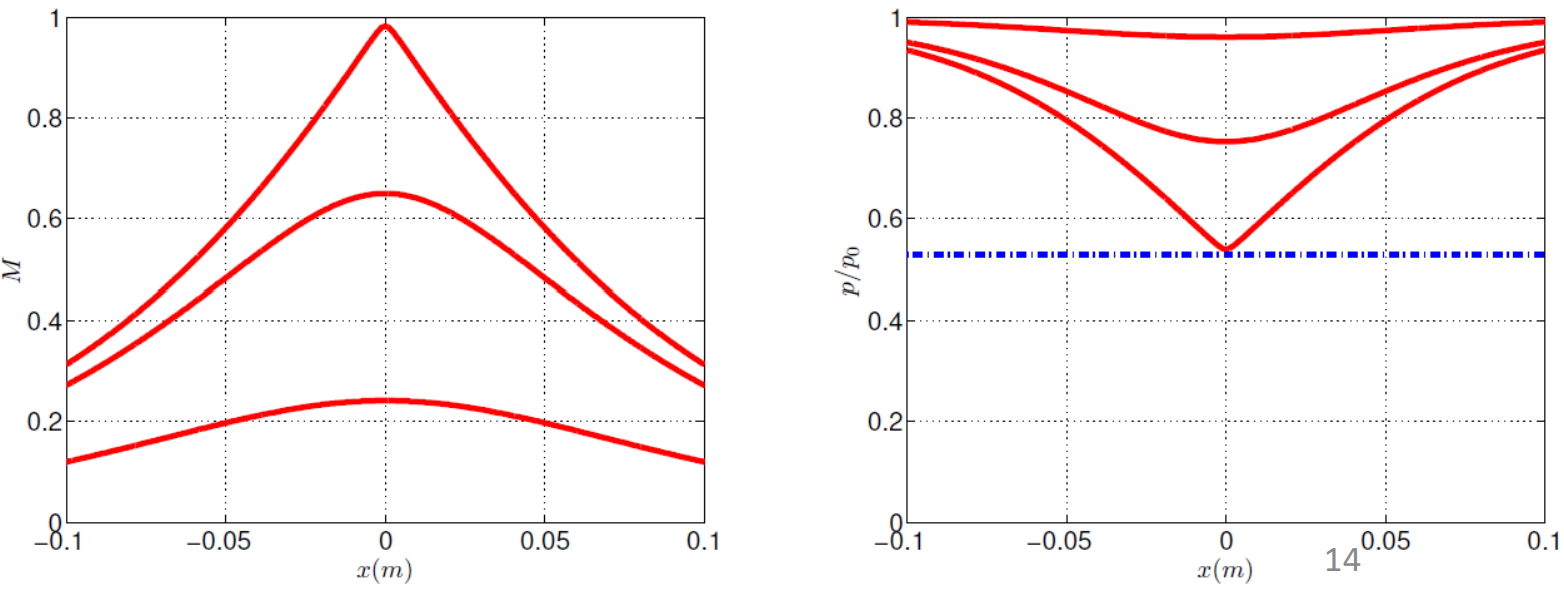
\includegraphics[width = 0.8\textwidth]{./img/diagram57.png}
\end{figure}
A more practical form of a flash ADC circuit can be achieved using voltage dividers, for the k-th comparator:
\begin{figure}[H]
  \centering
  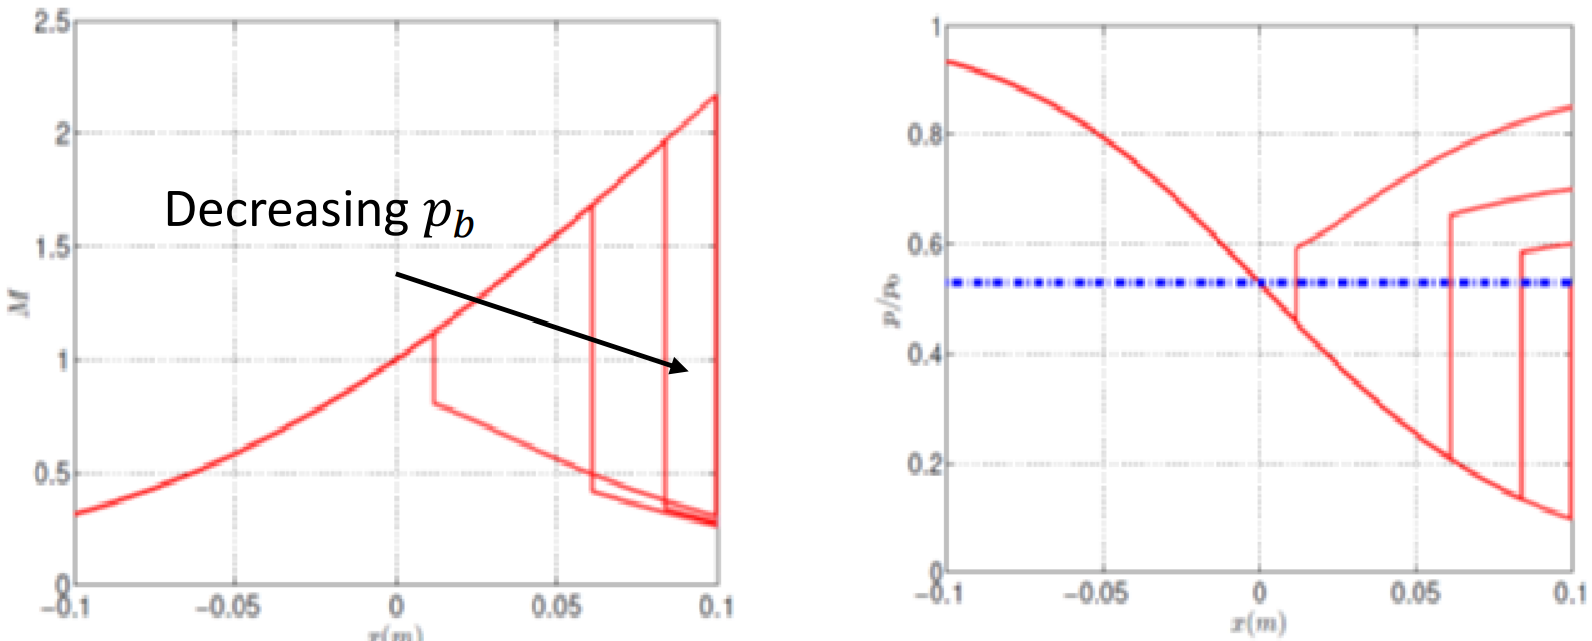
\includegraphics[width = 0.2\textwidth]{./img/diagram58.png}
\end{figure}
\begin{equation}
  V_{o, k} = A_v \left(V_{in} - \frac{\left(k + \frac{1}{2}\right)R}{nR} V_{REF}\right) \textrm{, } k = 1, \ 2, \ ..., \ n-1
\end{equation}
$n$ comparators allow judgement of YES/NO per every $V_{REF} / n$ volt $\rightarrow$ \textbf{resolution} of conversion.
\begin{itemize}
  \item 8-bit quantisation requires $2^8 = 256$ comparators.
  \item 16-bit quantisation requires $2^{16} = 25536$ comparators.
\end{itemize}
Flash ADC can work very quickly but becomes complex for high resolutions.
\subsection{Other types of ADC}
There are other types of conversion:
\begin{itemize}
  \item Successive conversion - successively narrow down range of $V_{in}$
  \item Integrating - use input signal integration time to find $V_{in}$
  \item Ramp-compare
\end{itemize}
Ramp-comparison utilises a saw tooth wave and the time period of switching to work out what $V_{in}$ is.
\begin{figure}[H]
  \centering
  \includegraphics[width = 0.8\textwidth]{./img/diagram59.png}
\end{figure}
\begin{equation}
  V_{in} = \frac{\Delta t}{T} V_{max}
\end{equation}
Ramp-compare can be done with a simply system (only one comparator) and can be accurate but may required (relatively - you can make the frequency of the sawtooth very large) long processing time.
\subsection{Typical issues to be considered}
\subsubsection*{Resolution}
Number of bits allocated to represent the input range (= interval of discrete data values).
\subsubsection*{Accuracy}
How the digitised values are different from the original values. E.g. affected by accuracy of $\Delta t$ measurement in ramp-compare. Though quantisation causes rounding error, it is not necessarily associated with accuracy.
\subsubsection*{Sampling rate}
How many data points over time (how many ADC per time period). Affected by ADC time. Particular impact on time-dependent data/frequency (e.g. music) leading to aliasing/anti-aliasing.
\subsubsection*{Noise}
Some methods (e.g. integrating) are good for noisy data.
\section{Interface devices to PC and programming platform}
\subsection{Arduino}
\begin{figure}[H]
  \centering
  \includegraphics[width = 0.8\textwidth]{./img/diagram60.png}
  \caption{Can be linked up with MATLAB or any other language.}
\end{figure}
\subsection{NI products and LabVIEW}
\begin{figure}[H]
  \centering
  \includegraphics[width = 0.8\textwidth]{./img/diagram61.png}
\end{figure}
\section{Experimental Errors}
Because of the inherent limitations of measurement equipment of techniques, there will always be some 'uncertainty' associated with experimental results. This uncertainty of error conveys significant information about the experiment and the result obtained, so you will be expected to assess the error in the measurements that you perform.
\subsubsection*{Example}
We want to know the volume of a cylinder based on diameter and height measurement:
\begin{equation}
  V = \pi r^2 h = \frac{\pi h d^2}{4}
\end{equation}
We must ask how accurate are $d$ and $h$, and also how they can be measured in the calculation of $V$? Suppose you are measuring a variable $x$:
\begin{figure}[H]
  \centering
  \includegraphics[width = 0.8\textwidth]{./img/diagram62.png}
  \caption{Actual error is mostly combination of both types of errors.}
\end{figure}
\subsection{Systematic errors}
Depends on:
\begin{itemize}
  \item Equipment
  \item Environment
        \begin{itemize}
          \item For example temperature may affect the measurement results, e.g. strain gauges. We deal with this by introducing temperature compensation.
        \end{itemize}
  \item Operator
        \begin{itemize}
          \item Consider measuring a sample with length $L$ and mass $M$. These are well defined variables, however the thickness $h$ will require sampling.
        \end{itemize}
\end{itemize}
\begin{figure}[H]
  \centering
  \includegraphics[width = 0.5\textwidth]{./img/diagram63.png}
  \caption{Sampling needs to be done carefully to ensure good representation.}
\end{figure}
Looping back to our cylinder example earlier, let us say:
\begin{align}
  d & = 8.2 \pm 0.5 \si{\centi\meter} \\
  h & = 9.5 \pm 0.2 \si{\centi\meter}
\end{align}
\subsection{Combining errors in a single quantity}
Uncertainty analysis / error propagation - Estimating the overall error in the measurement system. For example, when two resistors are connected in series, what is the expected uncertainty of the total resistance?
\begin{align}
  R_1 & = 1000 \pm 1.5 \si{\ohm} \\
  R_2 & = 500 \pm 1.0 \si{\ohm}
\end{align}
The straightforward option is to simply add them directly $\rightarrow 2.5\si{\ohm}$
\begin{equation}
  R_{total} = R_1 + R_2 = 1500 \pm 2.5 \si{\ohm}
\end{equation}
The error in $R_1$ and $R_2$ are a statistical indication, whereby the error is assumed to follow a Gaussian (normal) distribution. However, simple addition of the errors is too pessimistic! The two errors are independent and unlikely to show their maximum at the same time. If the errors are \textbf{independent} and in the same \textbf{quantity}, they can be combined as:
\begin{equation}
  E = \pm \sqrt{e_1^2 + e_2^2}
\end{equation}
and for this resistor example, overall error is $1.8 \si{\ohm}$. The rule above can be applied to any number of independent errors:
\begin{equation}
  E = \pm \sqrt{e_1^2 + e_2^2 + e_e^2 + ...}
\end{equation}
\subsection{Various combinations of quantities}
Assuming independent measurements $A$ and $B$, which have total errors $\Delta A$ and $\Delta B$ associated with them, are combined t o give the result $X$, which has error $\Delta X$, then:
\begin{align}
  \textrm{if } X = A + B \textrm{ or } X = A - B    & \longrightarrow \Delta X = \sqrt{(\Delta A)^2 + (\Delta B)^2}                                                     \\ \label{addsuberror}
  \textrm{if } X = AB \textrm{ or } X = \frac{A}{B} & \longrightarrow \frac{\Delta X}{X} = \sqrt{\left(\frac{\Delta A}{A}\right)^2 + \left(\frac{\Delta B}{B}\right)^2} \\
  \textrm{if } X = A^n                              & \longrightarrow \frac{\Delta X}{X} = n \frac{\Delta A}{A}                                                         \\
\end{align}
Note for equation (\ref{addsuberror}), we always use plus in our square root because the error only increases with addition or subtraction. When more than two quantities are involved, the equations are extended in a straightforward way:
\begin{align}
  \textrm{if } & X = A + B - C + D ... \longrightarrow \Delta X = \sqrt{(\Delta A)^2 + (\Delta B)^2 + (\Delta C)^2 + (\Delta D)^2}                                                                                           \\
  \textrm{if } & X = \frac{AB}{CD} \longrightarrow \frac{\Delta X}{X} = \sqrt{\left(\frac{\Delta A}{A}\right)^2 + \left(\frac{\Delta B}{B}\right)^2 + \left(\frac{\Delta C}{C}\right)^2 + \left(\frac{\Delta D}{D}\right)^2}
\end{align}
Adding errors in summation (A+B) and subtraction (A-B) are simpler because they must be the same physical quantity (mass, length, etc.) with the same unit. Products and divisions are usually in different quantity and the errors need to be added in normalised fashion. Let us use these in our cylinder example now:
\begin{gather}
  V = \pi r^2 h = \frac{\pi h d^2}{4}\\
  d = 8.2 \pm 0.5 \si{\centi\meter}\\
  h = 9.5 \pm 0.2 \si{\centi\meter}\\
  V = 387 \si{\centi\meter\cubed}
\end{gather}
Using two of the error estimation rules in combination,
\begin{equation}
  \frac{\Delta V}{V} = \sqrt{\left(\frac{\Delta h}{h}\right)^2 + \left(\frac{2\Delta d}{d}\right)^2} \longrightarrow \Delta V = 54 \si{\centi\meter\cubed}
\end{equation}
Therefore the volume is $V = 387 \pm 54 \si{\centi\meter\cubed}$
\subsection{General rule for combining errors}
Consider the problem of computing a quantity $N$, where $N$ is a known function of the n independent variables $u_1, \ u_2, \ u_3, \ ..., \ u_n$. That is:
\begin{equation}
  N = f(u_1, \ u_2, \ u_3, \ ..., \ u_n)
\end{equation}
The $u$s are the measured quantity with errors $\pm \Delta u_1, \ \pm \Delta u_2, \ \pm \Delta u_3, \ ..., \ \pm \Delta u_n$ which result in error in $N$. We could now write:
\begin{equation}
  N \pm \Delta N = f(u_1 \pm \Delta u_1, \ u_2 \pm \Delta u_2, \ u_3 \pm \Delta u_3, \ ..., \ u_n \pm \Delta u_n)
\end{equation}
Expanding $f$ in Taylor series we get:
\begin{multline}
  f(u_1 \pm \Delta u_1, \ u_2 \pm \Delta u_2, \ u_3 \pm \Delta u_3, \ ..., \ u_n \pm \Delta u_n) = \\
  f(u_1, \ u_2, \ u_3, \ ..., \ u_n) + \Delta u_1 \frac{\partial f}{\partial u_1} + \Delta u_2 \frac{\partial f}{\partial u_2} + ... + \Delta u_n \frac{\partial f}{\partial u_n} \\ + \textrm{higher order terms}
\end{multline}
Where $f(u_1, \ u_2, \ u_3, \ ..., \ u_n)$ is our $N$. We can neglect our higher order terms because $\Delta u_n << 1$ and what we are left with is our error.
\begin{equation}
  \textrm{Error } = \Delta u_1 \frac{\partial f}{\partial u_1} + \Delta u_2 \frac{\partial f}{\partial u_2} + ... + \Delta u_n \frac{\partial f}{\partial u_n}
\end{equation}
Considering $\Delta u$s are not absolute limits of error but rather as statistical bounds of uncertainties the proper method of combing the error is according to the root-sum square formula:
\begin{equation}
  E = \sqrt{\left(\Delta u_1 \frac{\partial f}{\partial u_1}\right)^2 + \left(\Delta u_2 \frac{\partial f}{\partial u_2}\right)^2 + ... + \left(\Delta u_n \frac{\partial f}{\partial u_n}\right)^2}
\end{equation}
\subsection{Example}
The resistance of a certain size of copper wire is given as
\begin{equation}
  R = R_0 [1 + \alpha (T-20)]
\end{equation}
Where $R_0 = 6\si{\ohm} \pm 0.3\%$ is the resistance at 20\si{\celsius}, $\alpha = 0.004 \si{\per\celsius} \pm 1\%$ is the temperature coefficient of resistance, and the temperature of the wire is $T = 30 \pm 1 \si{\celsius}$. Calculate the resistance of the wire and its uncertainty.

The nominal resistance is:
\begin{equation}
  R = 6 [1 + 0.004 \times (30 -20)] = 6.24 \si{\ohm}
\end{equation}
The uncertainty is from the equation earlier,
\begin{equation}
  \Delta R = \sqrt{\left(\Delta R_0 \frac{\partial R}{\partial R_0}\right)^2 + \left(\Delta \alpha \frac{\partial R}{\partial \alpha}\right)^2 + \left(\Delta T\frac{\partial R}{\partial T}\right)^2}
\end{equation}
Here,
\begin{align}
  \frac{\partial R}{\partial R_0}    & = 1 + \alpha (T-20)                \\
                                     & = 1 + 0.004 \times (30 -20) = 1.04 \\
  \frac{\partial R}{\partial \alpha} & = R_0 (T-20)                       \\
                                     & = 6 \times (30-20) = 60            \\
  \frac{\partial R}{\partial T}      & = R_0 \alpha                       \\
                                     & = 6 \times 0.004 = 0.024
\end{align}
And,
\begin{gather}
  \Delta R_0 = 6 \times 0.003 = 0.018 \si{\ohm}\\
  \Delta \alpha = 0.004 \times 0.01 = 4 \times 10^{-5} \si{\per\celsius}\\
  \Delta T = 1 \si{\celsius}
\end{gather}
Thus, the uncertainty in the resistance is:
\begin{equation}
  0.0305 \si{\ohm} \textrm{ or } 0.49 \%
\end{equation}
\subsection{What if we do not know the relationship between error sources and measured variables?}
Example: load cell (force measurement)
\begin{equation}
  V_0 = f(\textrm{load, etc})
\end{equation}
Simply add relevant errors up based on the specification sheet as a safety measure.
\section{Reference information about least-square curve fitting}
\subsection{Least square analysis}
The least squares method is often used to establish the functional relationship between the dependent measured variable and the independent process variable. In most situations, the anticipated relationship is polynomial. The variation found in the measured variable is assumed to follow a normal (Gaussian) distribution about each fixed value of the independent variable.
\begin{figure}[H]
  \centering
  \includegraphics[width = 0.5\textwidth]{./img/diagram64.png}
\end{figure}
Suppose two variables $x$ and $y$ are measured over a range of values. We want to find their mathematical relationship. The simplest polynomial function is linear: $y = ax + b$. Least square analysis is done by minimising the quantity:
\begin{equation}
  S = \sum_{i = 1}^n [ y_i - (ax_i +b)]^2
\end{equation}
This is the same as finding:
\begin{equation}
  \frac{\partial S}{\partial a} = 0, \ \frac{\partial S}{\partial b} = 0
\end{equation}
\begin{figure}[H]
  \centering
  \includegraphics[width = 0.5\textwidth]{./img/diagram65.png}
\end{figure}
\begin{align}
  \frac{\partial S}{\partial a} = \sum_{i = 1}^n (2 ax_i^2 + 2bx_i - 2x_i y_i) = 0 & \rightarrow a\sum_{i=1}^n x_i^2 + b\sum_{i +1}^n x_i = \sum_{i=1}^n x_i y_i \\
  \frac{\partial S}{\partial b} = \sum_{i=1}^n (2ax_i + 2b - 2y_i)                 & \rightarrow a\sum_{i=1}^n x_i + nb = \sum_{i=1}^n y_i
\end{align}
\begin{gather}
  a = \frac{n \sum_{i=1}^n x_i y_i - \left(\sum_{i=1}^n x_i\right)\left(\sum_{i=1}^n y_i\right)}{n\sum_{i=1}^n x_i^2 - \left(\sum_{i=1}^n x_i\right)^2}\\
  b = \frac{\left(\sum_{i=1}^n x_i^2\right) \left(\sum_{i=1}^n y_i\right) - \left(\sum_{i=1}^n x_i y_i\right)\left(\sum_{i=1}^n x_i\right)}{n\sum_{i=1}^n x_i^2 - \left(\sum_{i=1}^n x_i\right)^2}
\end{gather}
Even with higher order polynomials, for example
\begin{equation}
  y = ax^2 + bx + c
\end{equation}
We can define quantity
\begin{equation}
  S = \sum_{i=1}^n [y_i - (ax_i^2 + bx_i +c)]^2
\end{equation}
for minimisation.
\begin{figure}[H]
  \centering
  \includegraphics[width = 0.5\textwidth]{./img/diagram66.png}
\end{figure}